\def\QRCODE{TB_image_TUT.IMG.image_enhancement_pythonqrcode.png}
\def\QRPAGE{http://www.iptutorials.science/tree/master/TB_image/TUT.IMG.image_enhancement/python}
\pcorrectionsection{Python correction}

\begin{python}
from scipy import misc
import matplotlib.pyplot as plt
from skimage import exposure
import numpy as np
import sys
\end{python}

\vspace*{-0.3cm}

\subsection{Intensity transformations}

\vspace*{-0.2cm}

\subsubsection{$\gamma$ correction}
\textls[-29]{The function \pinline{skimage.exposure.adjust_gamma} is used in order to adjust the gamma of the image. It is before normalized (values are float between 0 and 1). The results are illustrated in Fig.\ref{fig:enhancement:python:gamma}.}
\begin{python}
I=imageio.imread("osteoblaste.png")
I = I / np.max(I);

gamma=2;
I2= exposure.adjust_gamma(I, gamma);
plt.imshow(I2);
plt.show();
\end{python}

\vspace*{-0.3cm}

\begin{figure}[H]
 \centering\caption{Gamma transforms.}%
 \subfloat[Original image.]{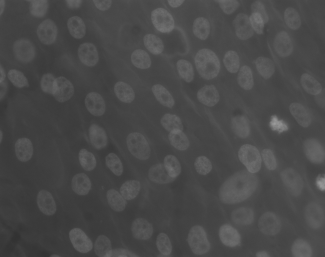
\includegraphics[width=.42\linewidth]{osteoblaste.png}}
 \hfill
 \subfloat[$\gamma=1$.]{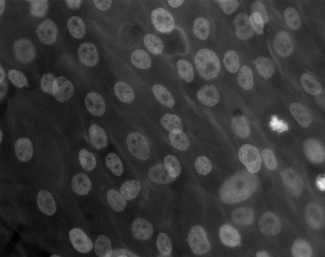
\includegraphics[width=.42\linewidth]{osteo_g1.png}}
 
 \subfloat[$\gamma=2$.]{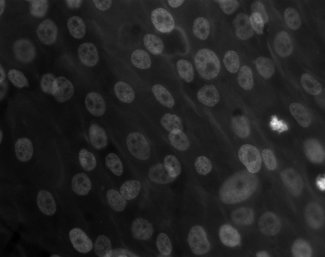
\includegraphics[width=.42\linewidth]{osteo_g2.png}} \hfill
 \subfloat[$\gamma=0.5$.]{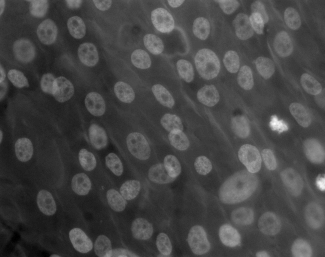
\includegraphics[width=.42\linewidth]{osteo_g05.png}}%
 \vspace*{-5pt}%
 \label{fig:enhancement:python:gamma}%
\end{figure}

\subsubsection{Contrast stretching}
The LUT look-up-table is simply a function applied to the original image. In order to avoid division by zero, the smallest float value is introduced. Fig.\ref{fig:enhancement:python:stretching} illustrates the results.

\begin{python}
def contrast_stretching(I, E):
    epsilon = sys.float_info.epsilon;
    m = np.mean(I);
    I = I.astype("float");
    Ar = 1. / (1.+(m/(I+epsilon))**E);
    return Ar;
\end{python}


\begin{figure}[htbp]
 \centering\caption{Constrast stretching.}%
 \subfloat[Original image.]{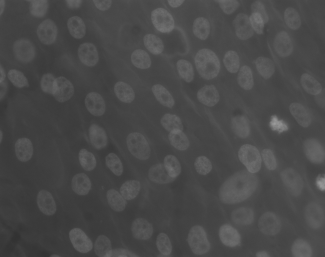
\includegraphics[width=.38\linewidth]{osteoblaste.png}} \hfill
 \subfloat[$E=10$.]{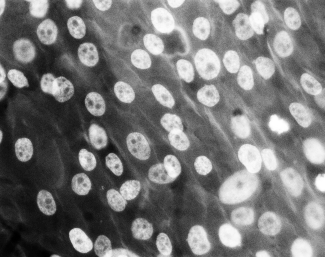
\includegraphics[width=.38\linewidth]{osteo_E10.png}}
 
 \subfloat[$E=20$.]{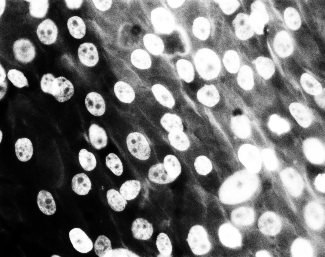
\includegraphics[width=.38\linewidth]{osteo_E20.png}} \hfill
 \subfloat[$E=1000$.]{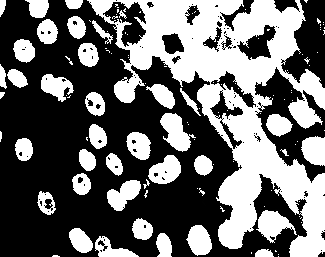
\includegraphics[width=.38\linewidth]{osteo_E1000.png}}%
 \vspace*{-5pt}%
 \label{fig:enhancement:python:stretching}%
\end{figure}
 \vspace*{-6mm}
\subsection{Histogram equalization}
The histogram is displayed with the following function:
\begin{python}
def displaySaveHisto(I, filename=None):
    """
    Display and save pdf (if filename provided) of histogram of image I
    If values are between 0 and 1, they are multiplied by 255
    """
    if np.max(I)<=1:
        I = 255 * I;
    hist,bins = np.histogram(I.flatten(), 256, range=(0,255))
    fig = plt.figure()
    plt.bar(bins[:-1], hist, width=1);
    plt.show();
    if filename!=None:
        fig.savefig(filename, bbox_inches='tight')
\end{python}

The histogram equalization is done via the \pinline{skimage.exposure.equalize_hist} function. The results are illustrated in Fig.\ref{fig:enhancement:python:histeq}.

\begin{python}
# histogram equalization
I2 = exposure.equalize_hist(I);
plt.imshow(I2);
plt.show()
\end{python}

The look-up-table (LUT) or cumulative distribution function (cdf) is computed and used in the next function:
\begin{python}
def histeq(I):
    """
    histogram equalization, version with look-up-table
    I: original image, with values in 8 bits integer
    """
    hist,bins=np.histogram(I.flatten(), 256, range=(0,255))
    cdf = hist.cumsum();
    cdf = (cdf / cdf[-1]);
    return cdf[I];
\end{python}

\vspace*{-0.5cm}

\begin{figure}[H]
 \centering\caption{Histogram equalization.}%
 \subfloat[Original image.]{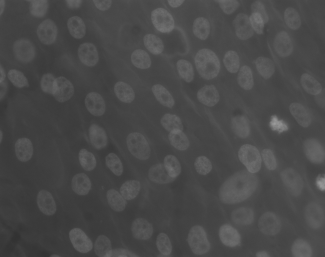
\includegraphics[width=.38\linewidth]{osteoblaste.png}}\hfill
 \subfloat[Histogram equa\-li\-za\-tion.]{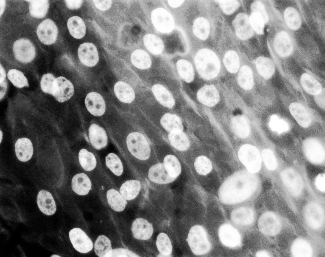
\includegraphics[width=.38\linewidth]{histeq_osteo.png}}
 
 \subfloat[Histogram of ori\-gi\-nal ima\-ge.]{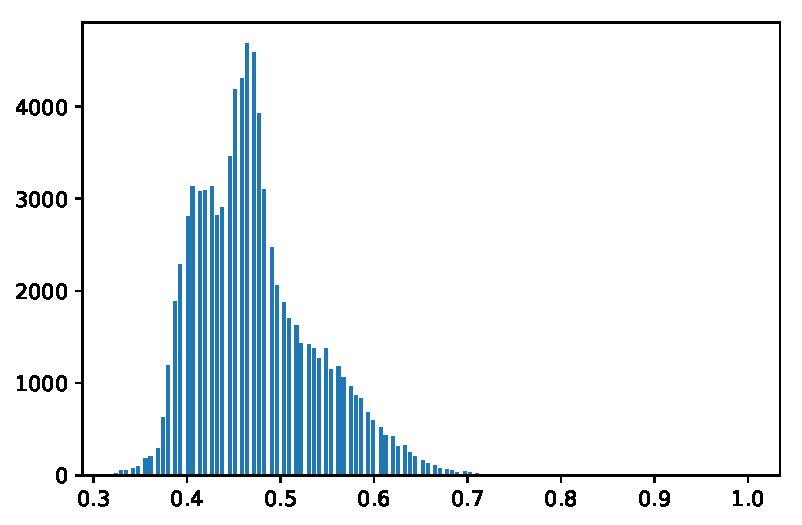
\includegraphics[width=.38\linewidth]{histo.pdf}}\hfill
 \subfloat[Histogram after equalization.]{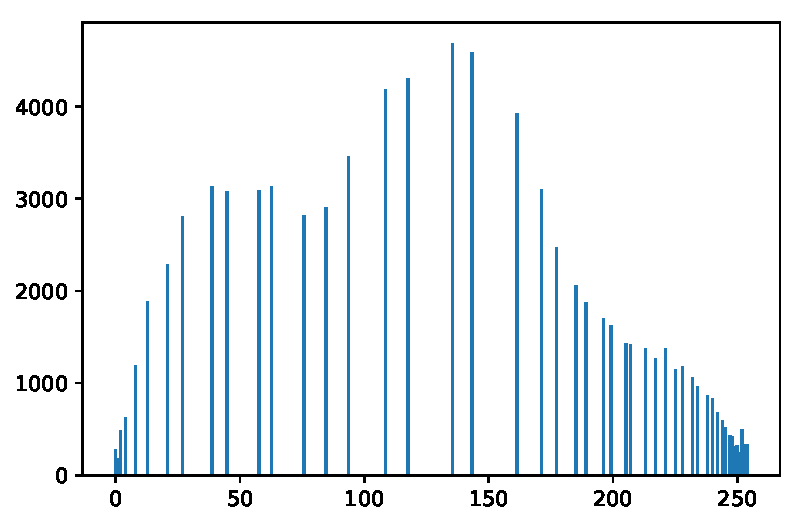
\includegraphics[width=.38\linewidth]{histeq_osteo_histo.pdf}}
 
  \vspace*{-7pt}
 
 \subfloat[LUT (cumulative distribution function).]{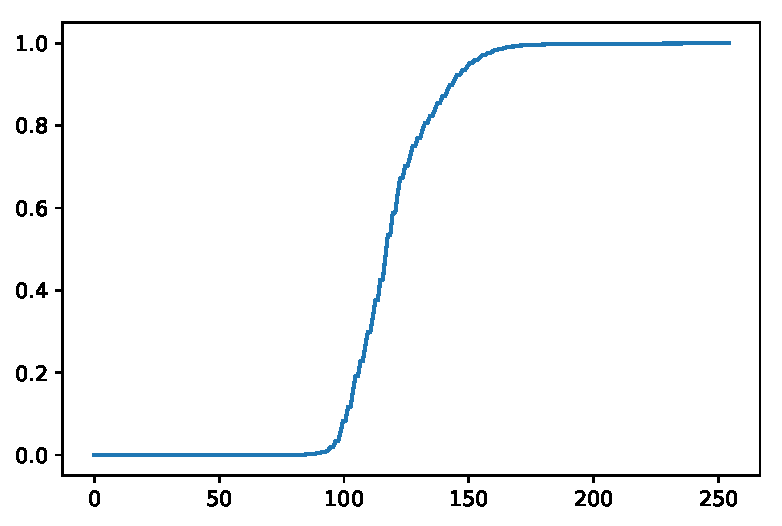
\includegraphics[width=.3\linewidth]{lut.pdf}\phantom{aaaaaaa}}%
 \vspace*{-10pt}%
 \label{fig:enhancement:python:histeq}%
\end{figure}

\subsection{Histogram matching}
\textls[-10]{This method is only an approximate method. It requires an interpolation of the cumulative distribution functions in order to find the transformation. Results are shown in Fig.\ref{fig:enhancement:python:histmatch}}

\begin{python}
def hist_matching(I, cdf_dest):
    """
    Histogram matching of image I, with cumulative histogram cdf_dest
    This should be normalized, between 0 and 1.
    This version uses interpolation
    """
    imhist,bins = np.histogram(I.flatten(), len(cdf_dest), density=True)
    cdf = imhist.cumsum() #cumulative distribution function
    cdf = (cdf / cdf[-1]) #normalize between 0 and 1
    # first: histogram equalization
    im2 = np.interp(I.flatten(), bins[:-1], cdf)
    # 2nd: reverse function
    im3 = np.interp(im2, cdf_dest, bins[:-1])
    # reshape into image 
    imres = im3.reshape(I.shape)
    return imres;
\end{python}

\begin{figure}[H]
 \centering\caption{Histogram matching.}%
 \subfloat[Original image.]{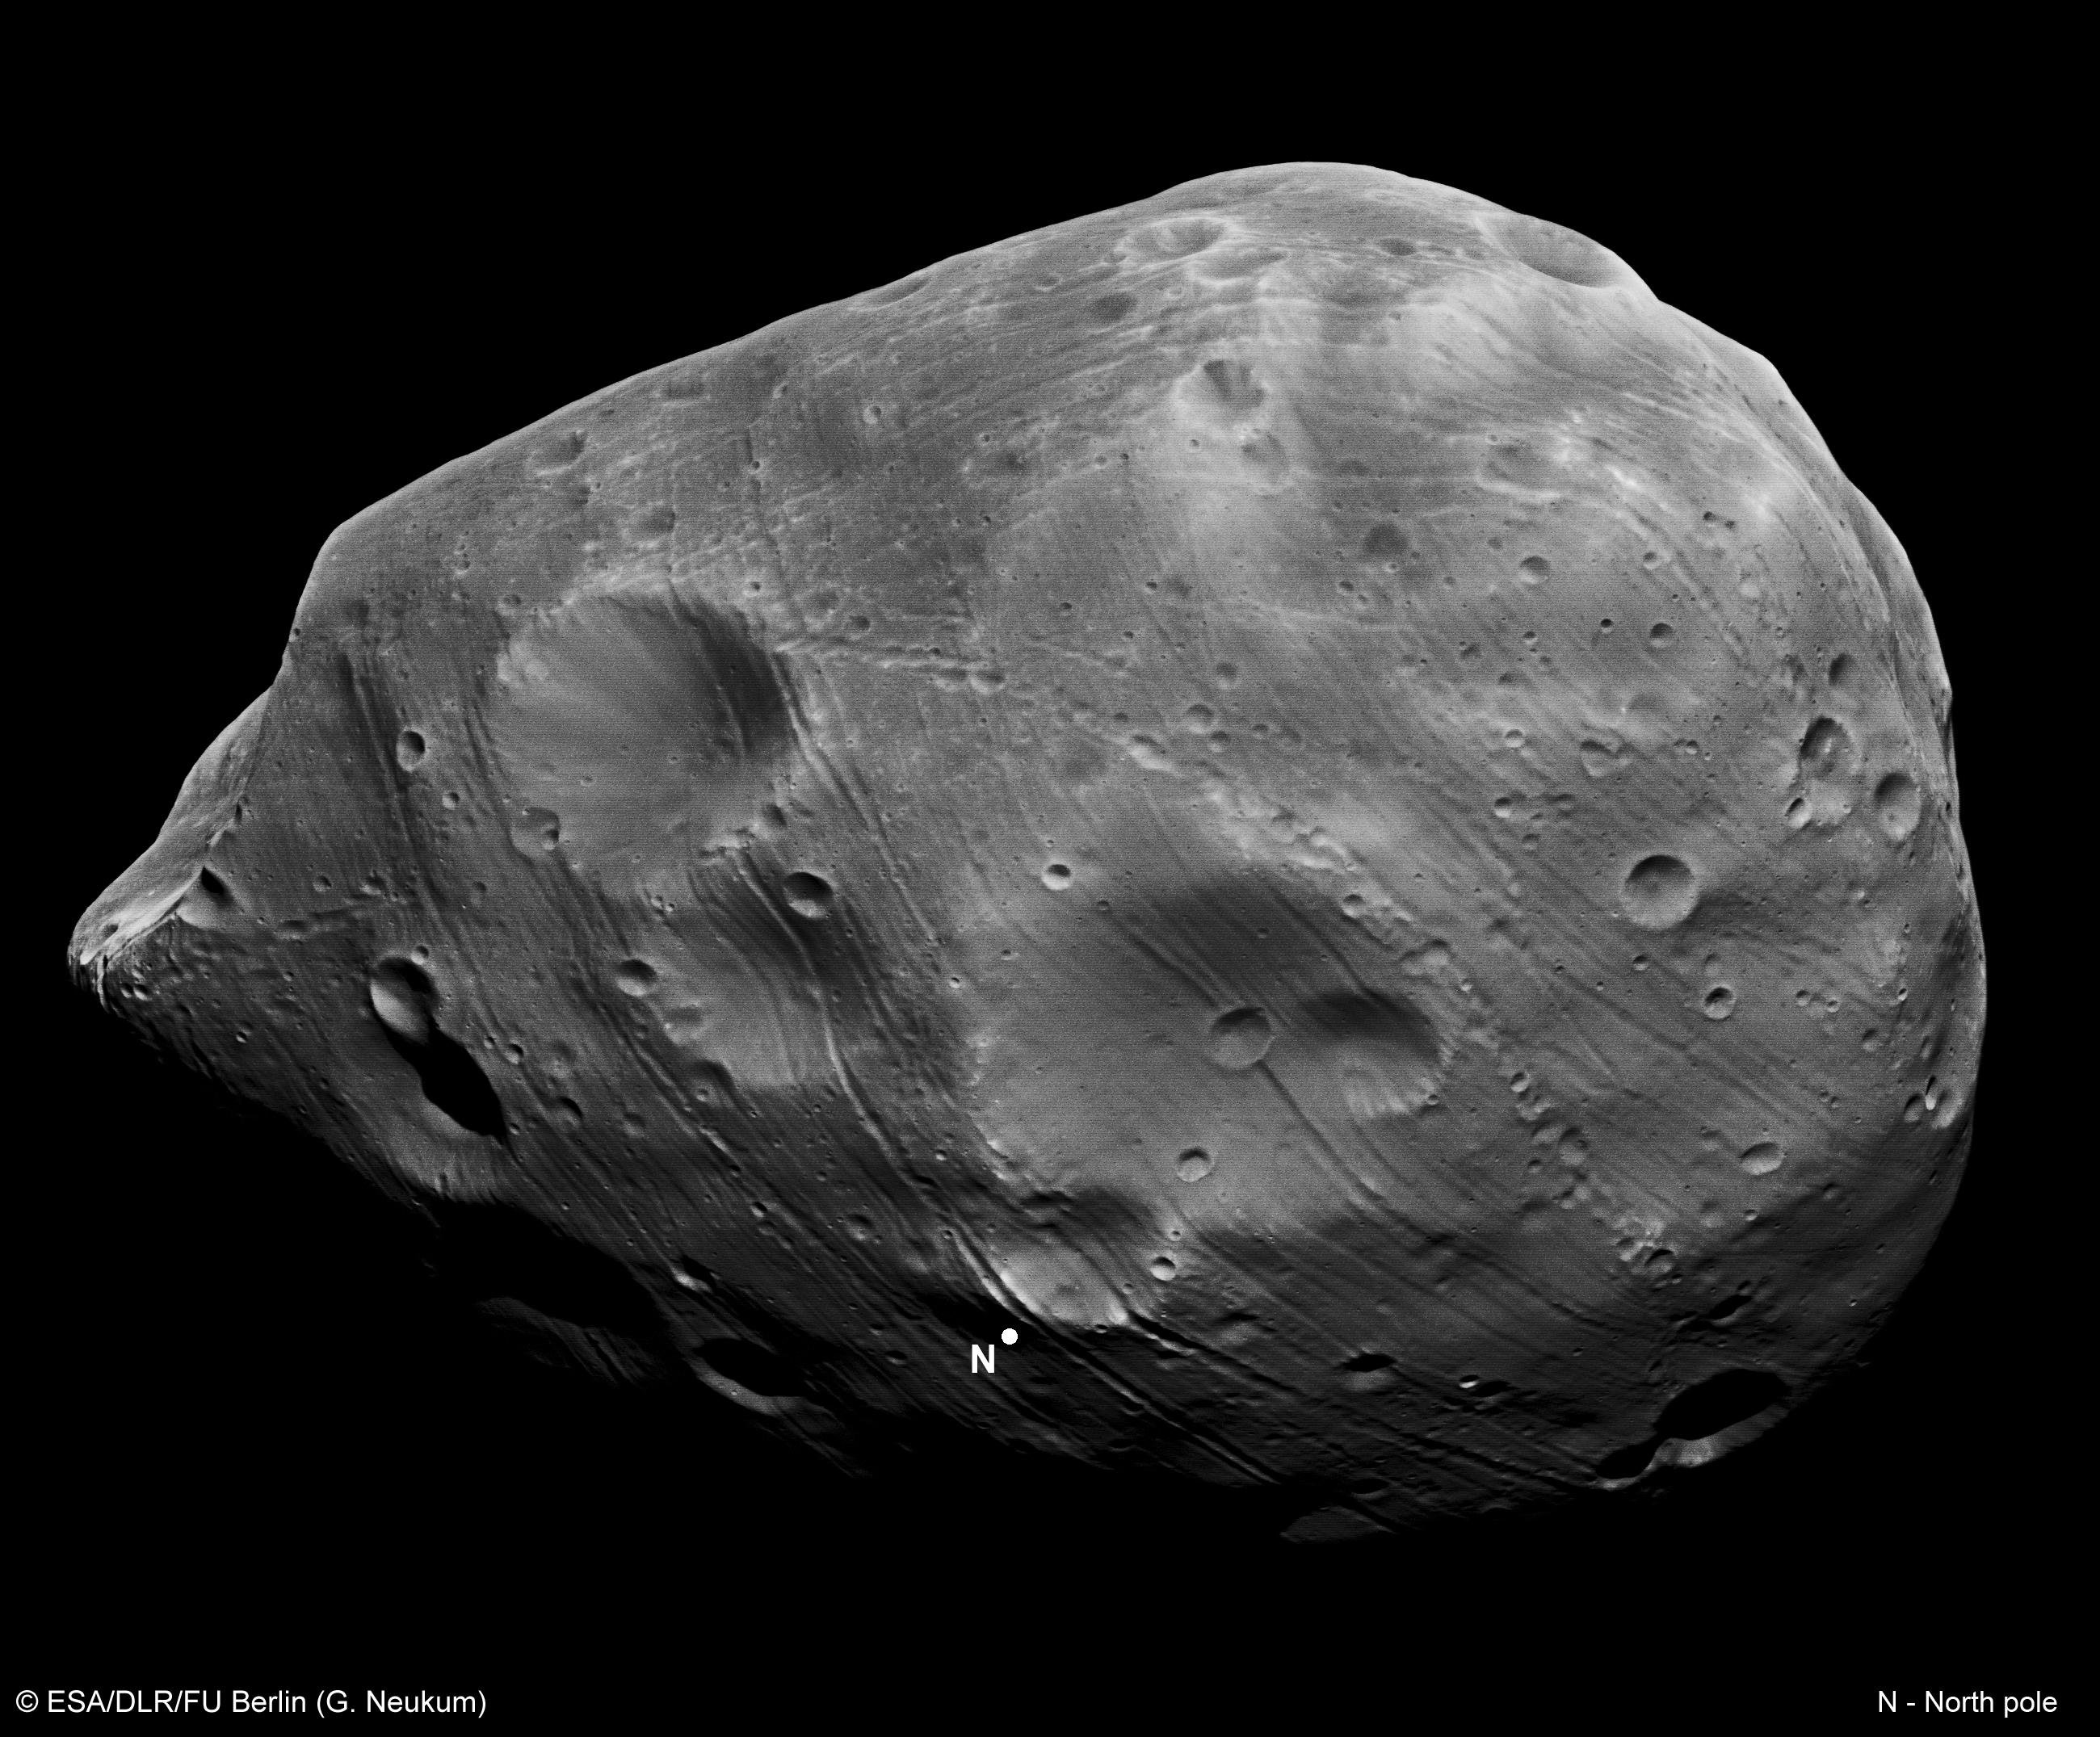
\includegraphics[width=.3\linewidth]{phobos.jpg}}\hfill
 \subfloat[Histogram equali\-za\-tion.]{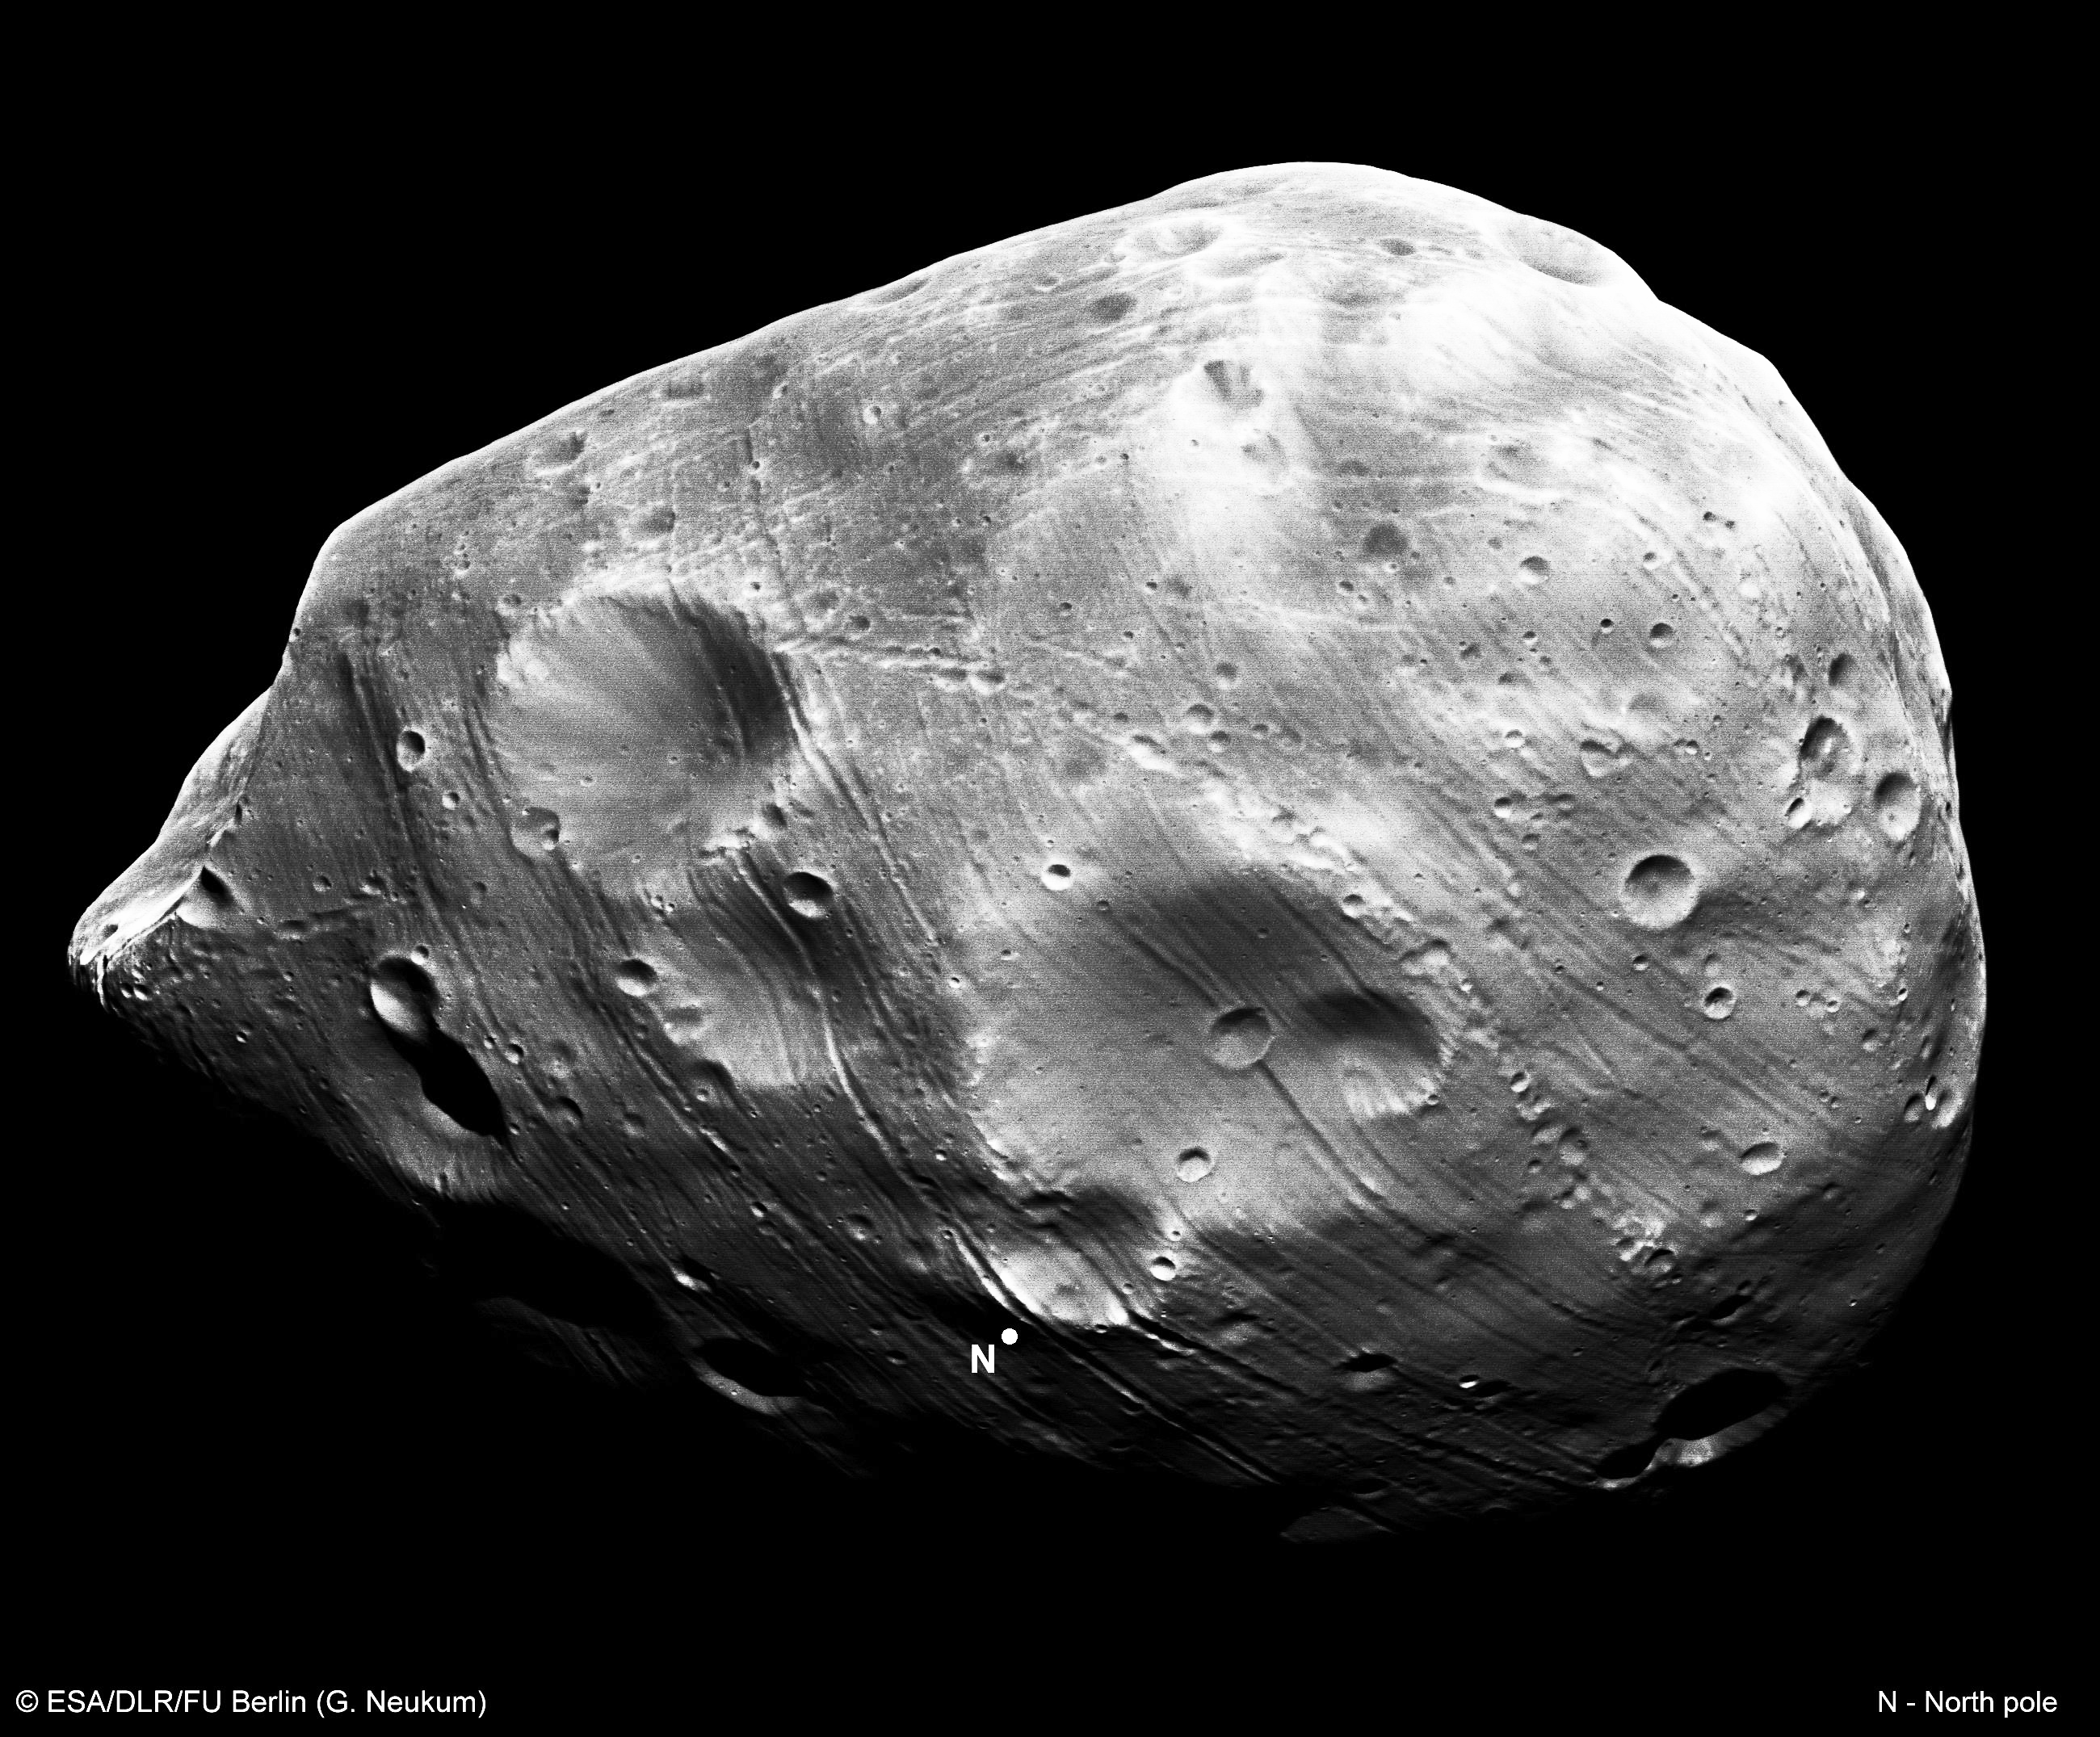
\includegraphics[width=.3\linewidth]{phobos_histeq.png}}\hfill
 \subfloat[Histogram matching.]{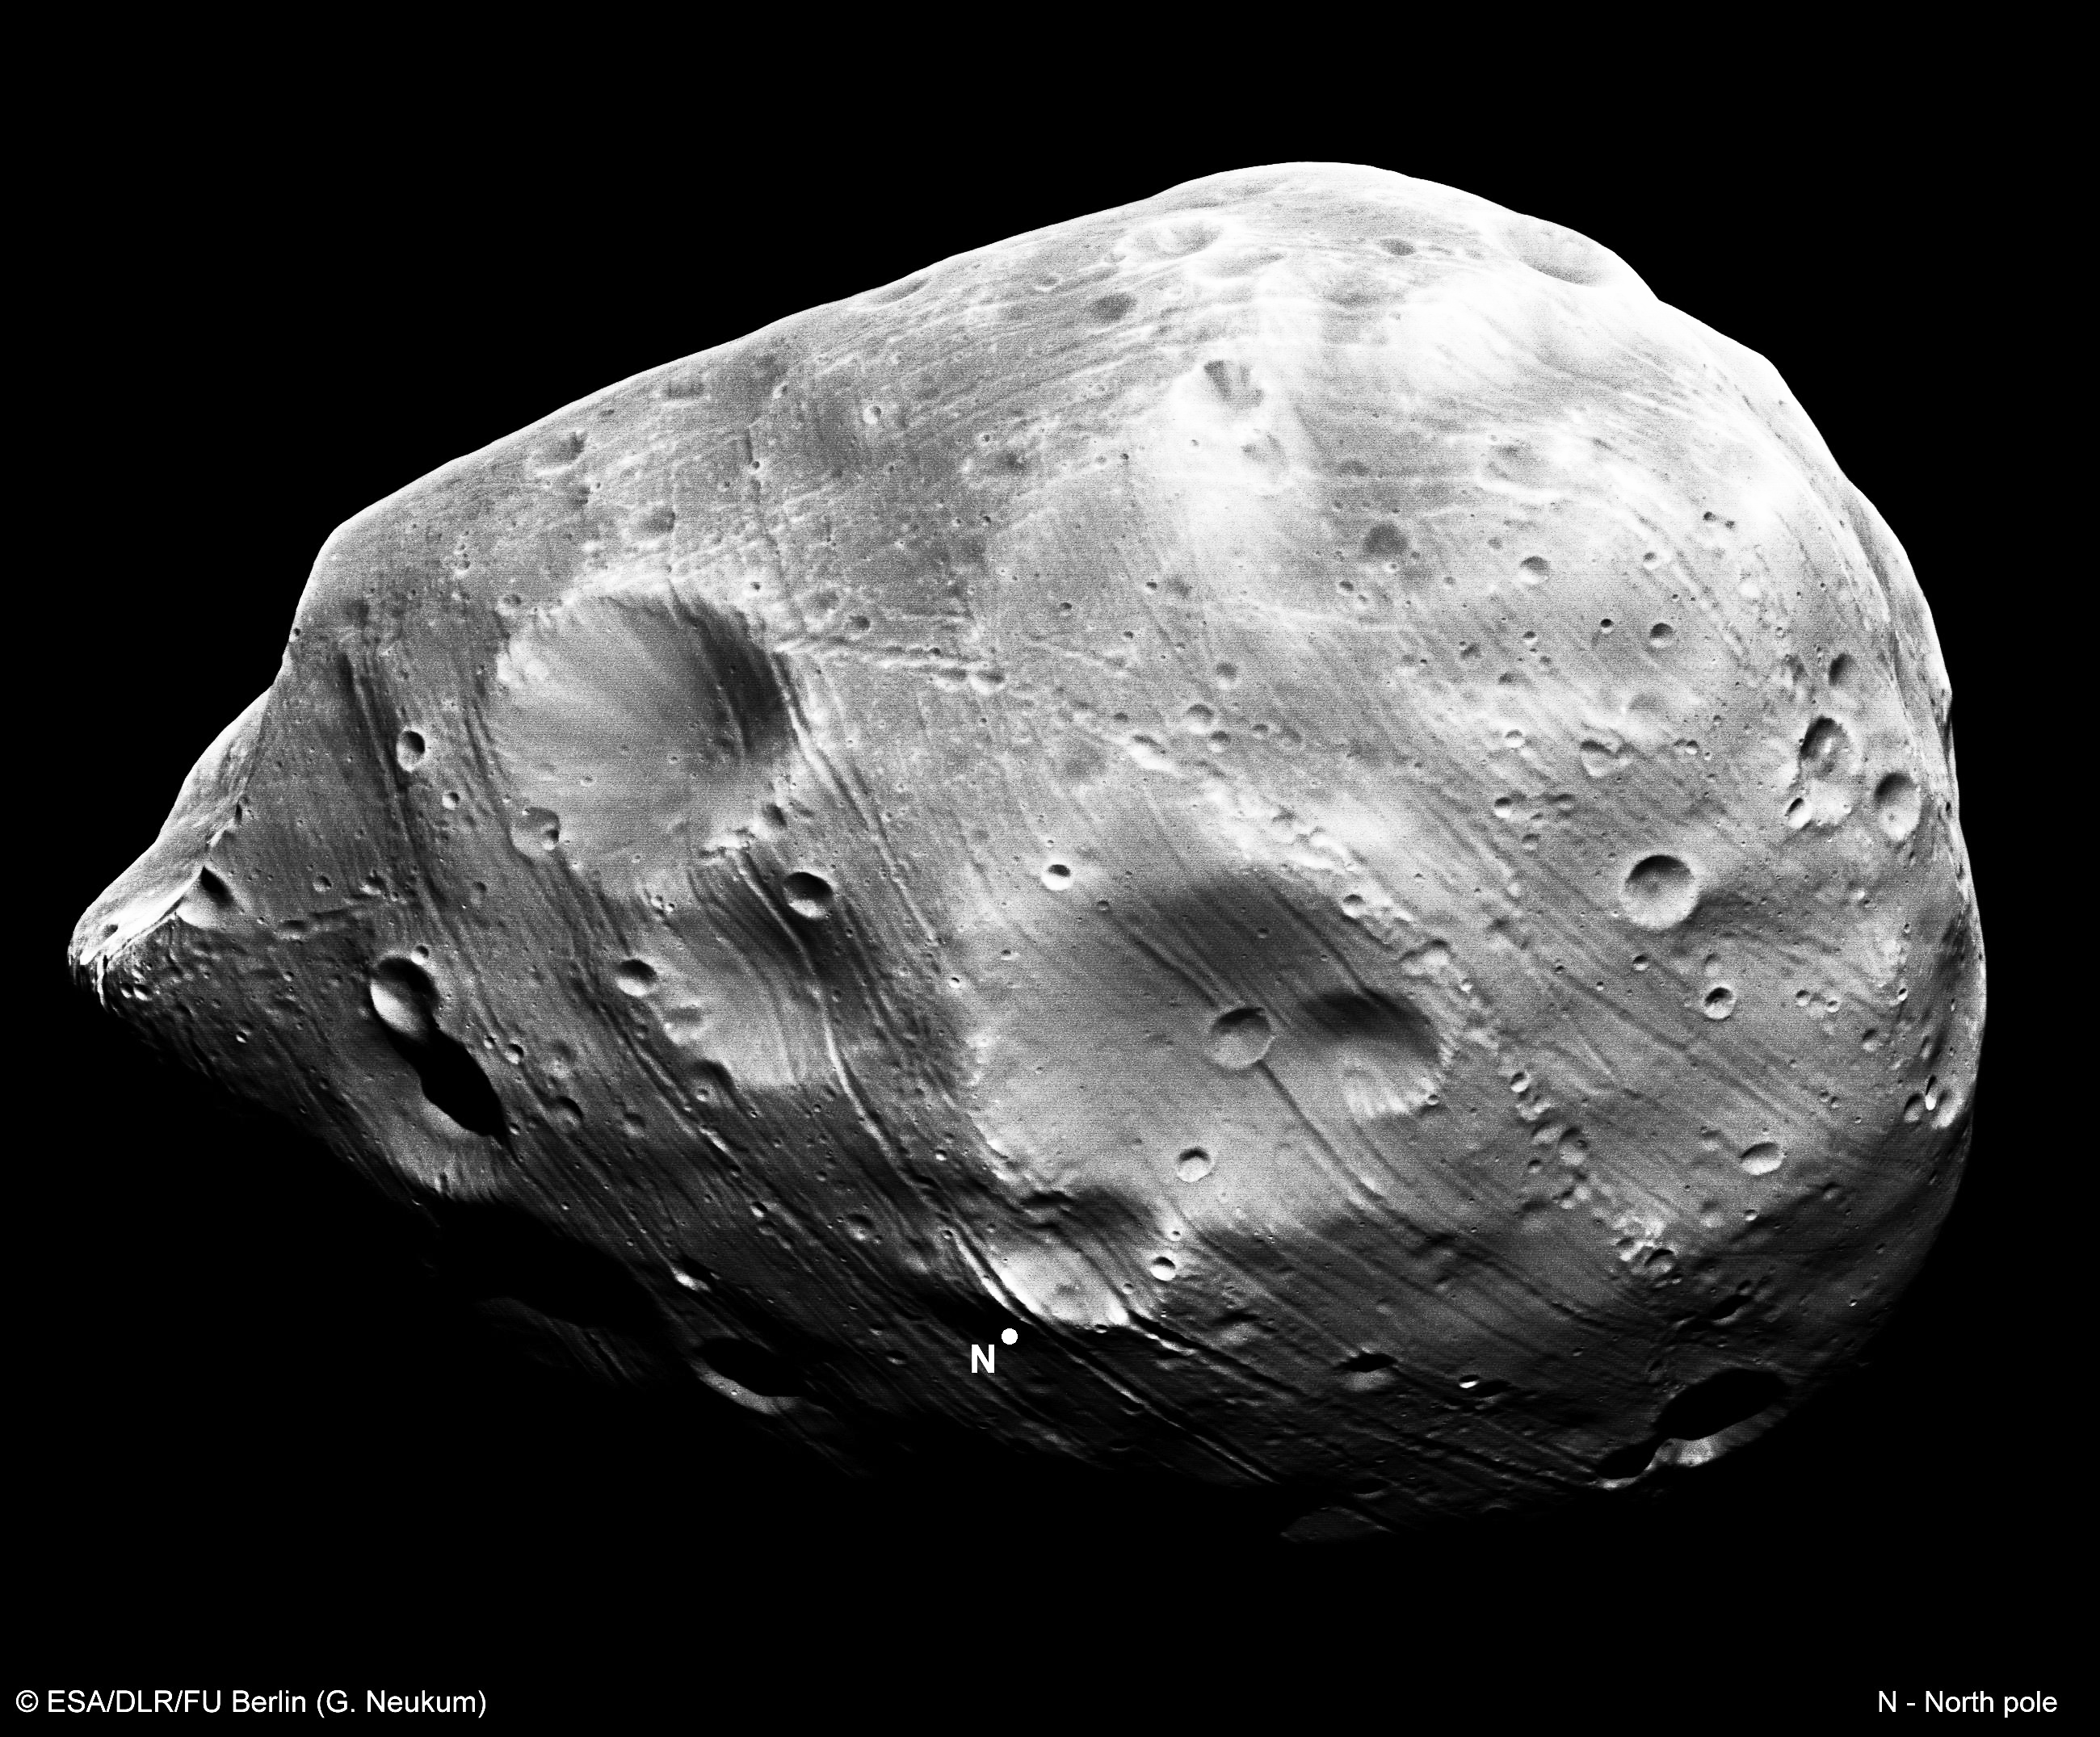
\includegraphics[width=.3\linewidth]{phobos_histmatch.png}}
 
 \vspace*{-5pt}
 
 \subfloat[Histogram of ori\-gi\-nal ima\-ge.]{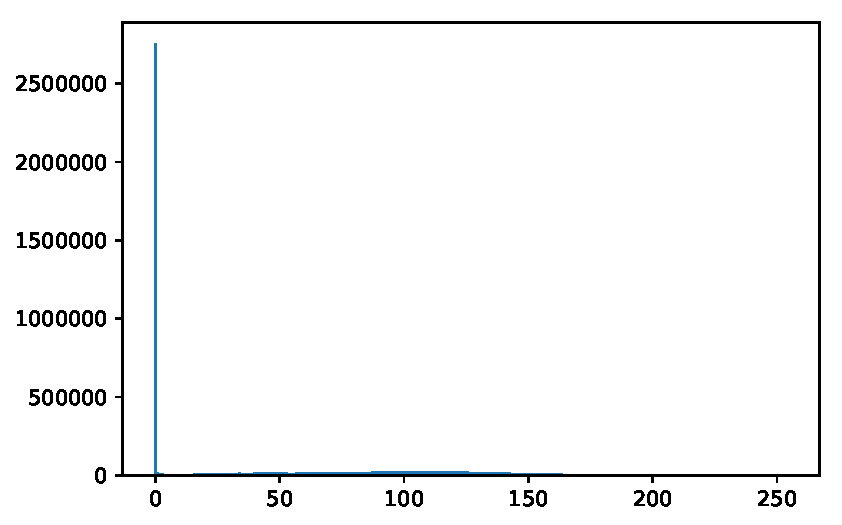
\includegraphics[height=3cm]{hist_phobos.pdf}}\hfill
 \subfloat[Histogram after equalization.]{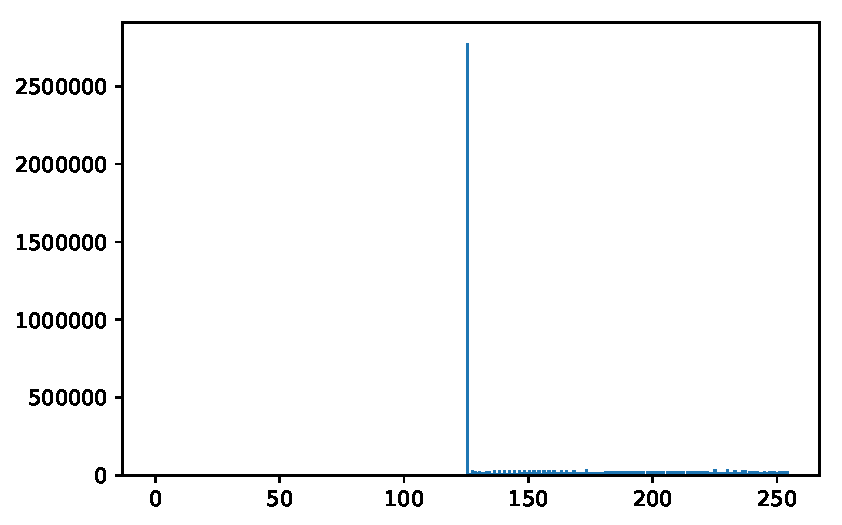
\includegraphics[height=3cm]{hist_phobos_histeq.pdf}}
 
  \vspace*{-5pt}

 \subfloat[Target histogram (cumulative distribution function).]{\hskip0.9cm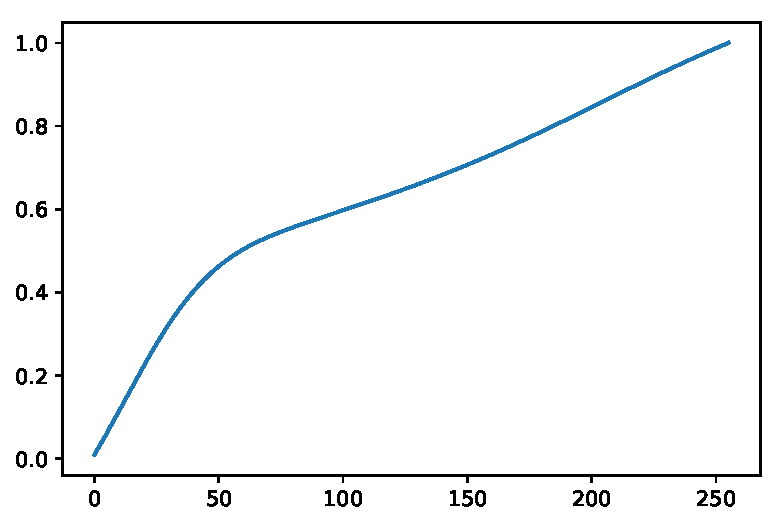
\includegraphics[height=2.9cm]{twomodegauss.pdf}}\hfill
 \subfloat[Histogram after histogram matching.]{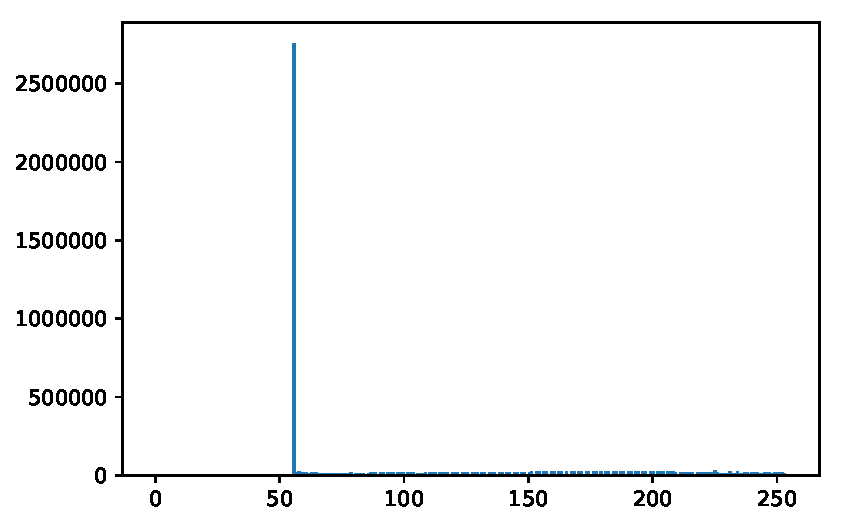
\includegraphics[height=3cm]{hist_phobos_matching.pdf}}%
 \label{fig:enhancement:python:histmatch}%
\end{figure}